\documentclass[aspectratio=169]{beamer}

% 中文支持
\usepackage[UTF8]{ctex}

% 数学相关宏包
\usepackage{amsmath,amssymb,enumerate}

% PPT 主题
\usetheme{Madrid}

% 字体设置
\setCJKmainfont{KaiTi}
\setCJKsansfont{KaiTi}
\setCJKmonofont{KaiTi}
	\title{这就是开源}
\subtitle{第一讲：从操作系统到开源}
\author{潘宇琦\hspace*{1em}申鹏威}
\begin{document}

\begin{frame}
	\title{这就是开源}
	\subtitle{第一讲：从操作系统到开源}
	\author{潘宇琦\hspace*{1em}申鹏威}
	\date{2026年10月}
	\titlepage
\end{frame}
	
\begin{frame}{}
	
\end{frame}
\begin{frame}{计算机里面有什么？}
\begin{block}{随便抓来一台电脑}
\begin{itemize}
	\item 处理器(CPU):厨师，按照菜谱做菜(执行程序)
	\item 内存(RAM)：案板，临时放置正在处理的食材(正在运行的程序)
	\item 硬盘(Disk)：冰箱and橱柜，长期保存食材和菜谱(文件与程序)
\end{itemize}
\end{block}

\begin{columns}[c,onlytextwidth]
\begin{column}{0.32\textwidth}
	\centering
	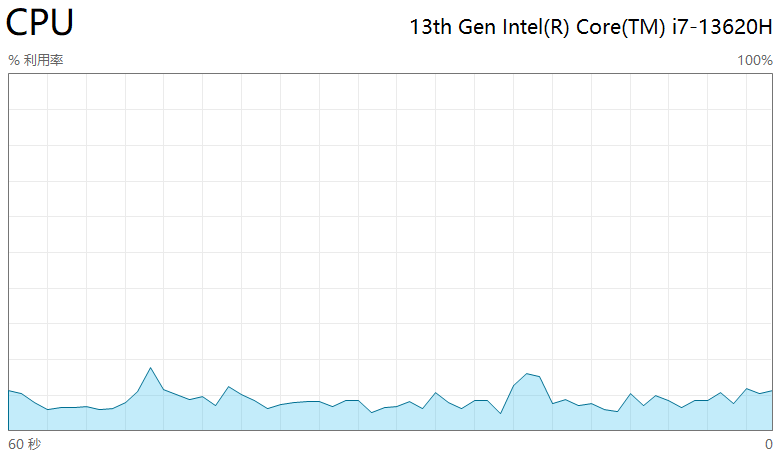
\includegraphics[
	width=\linewidth,
	height=3cm,
	keepaspectratio
	]{images/1.png}
\end{column}
	
\begin{column}{0.32\textwidth}
	\centering
	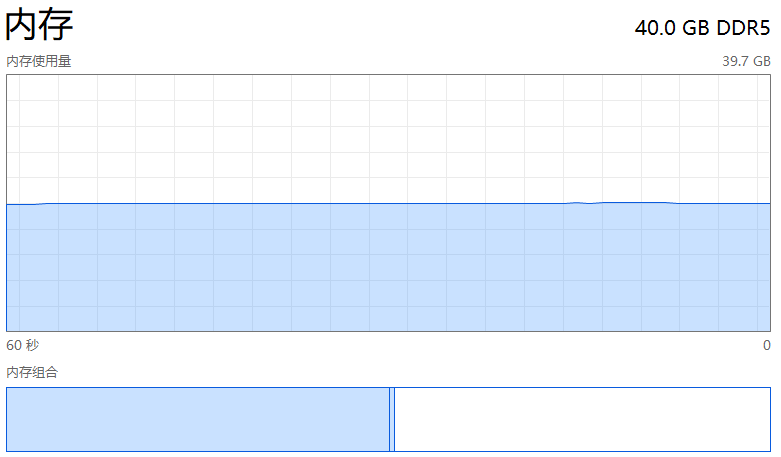
\includegraphics[
	width=\linewidth,
	height=3cm,
	keepaspectratio
	]{images/2.png}
\end{column}
	
\begin{column}{0.32\textwidth}
	\centering
	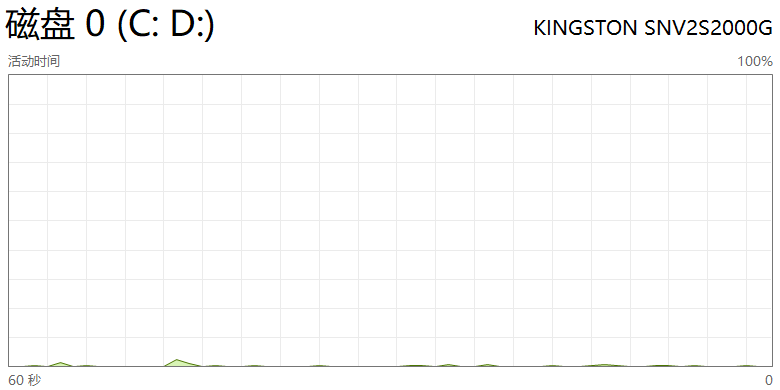
\includegraphics[
	width=\linewidth,
	height=3cm,
	keepaspectratio
	]{images/3.png}
\end{column}
\end{columns}
\end{frame}

\begin{frame}{为什么我们需要操作系统}
\begin{block}{如果你正在使用电脑...}
\hspace*{2em}这时，你的导员在QQ上给你发了文件，你的部长在微信上给你发了通知，你的同学在抖音上给你转发了视频...那处理器该先给谁用呢？内存该怎么分配呢？

\par\hspace*{2em}我们既想让它们运行又不想让它们挤破头，该怎么办呢？
\end{block}

\begin{block}{我们需要一个管理者！}
\hspace*{2em}就像厨房需要厨师长安排厨师的工作、分配厨具的使用一样，计算机也需要一个管理者，负责协调各个程序对硬件资源的使用。

\par\hspace*{2em}它要安排程序何时使用处理器、合理分配内存，还要尽可能避免不同程序之间的相互干扰。

\par\hspace*{2em}\alert{这个管理者，就是操作系统（Operating System，OS）。}
\end{block}
\end{frame}

\begin{frame}{为什么我们需要操作系统}
	
	\begin{block}{当有人在微信上给你发送了一张图片}
		\hspace*{2em}当你点击“保存”时，程序需要将图片保存到硬盘上。但程序应该怎样操作硬盘呢？
	\end{block}
	
	\begin{columns}[T,onlytextwidth]
		\begin{column}{0.48\textwidth}
			\begin{block}{没有统一的系统服务}
				程序需要自行处理存储设备的操作细节，甚至适配不同的硬件。
			\end{block}
		\end{column}
		
		\begin{column}{0.48\textwidth}
			\begin{block}{有操作系统提供服务}
				程序只需要请求“写入文件”，操作系统就可以帮助完成底层操作。
			\end{block}
		\end{column}
	\end{columns}
	
	\begin{block}{保存图片的过程（简化）}
		\centering
		微信
		$\longrightarrow$
		操作系统
		$\longrightarrow$
		存储设备
	\end{block}
	
	\vspace{0.3cm}
	
	\begin{center}
		\alert{操作系统为应用程序提供统一的服务，让程序不必直接处理复杂的硬件细节。}
	\end{center}
	
\end{frame}

\begin{frame}{什么是OS}
	\begin{block}{操作系统（Operating System，OS）}
		\hspace*{2em}操作系统是管理计算机硬件与软件资源，并为应用程序提供运行环境和基础服务的系统软件。
	\end{block}
		
	\begin{columns}[T,onlytextwidth]
		\begin{column}{0.48\textwidth}
			\begin{block}{资源管理者}
				\begin{itemize}
					\item 安排处理器工作
					\item 分配内存空间
					\item 管理文件与设备
				\end{itemize}
			\end{block}
		\end{column}
			
		\begin{column}{0.48\textwidth}
			\begin{block}{程序服务者}
				\begin{itemize}
					\item 帮助程序读写文件
					\item 提供统一的设备接口
					\item 为程序提供运行环境
				\end{itemize}
			\end{block}
		\end{column}
	\end{columns}
		
	\begin{center}
		\alert{操作系统既是资源的管理者，也是连接应用程序与计算机硬件的桥梁。}
	\end{center}
\end{frame}

\begin{frame}{操作系统发展史}
	
\begin{block}{世界早期的电子计算机——ENIAC}
	\centering
	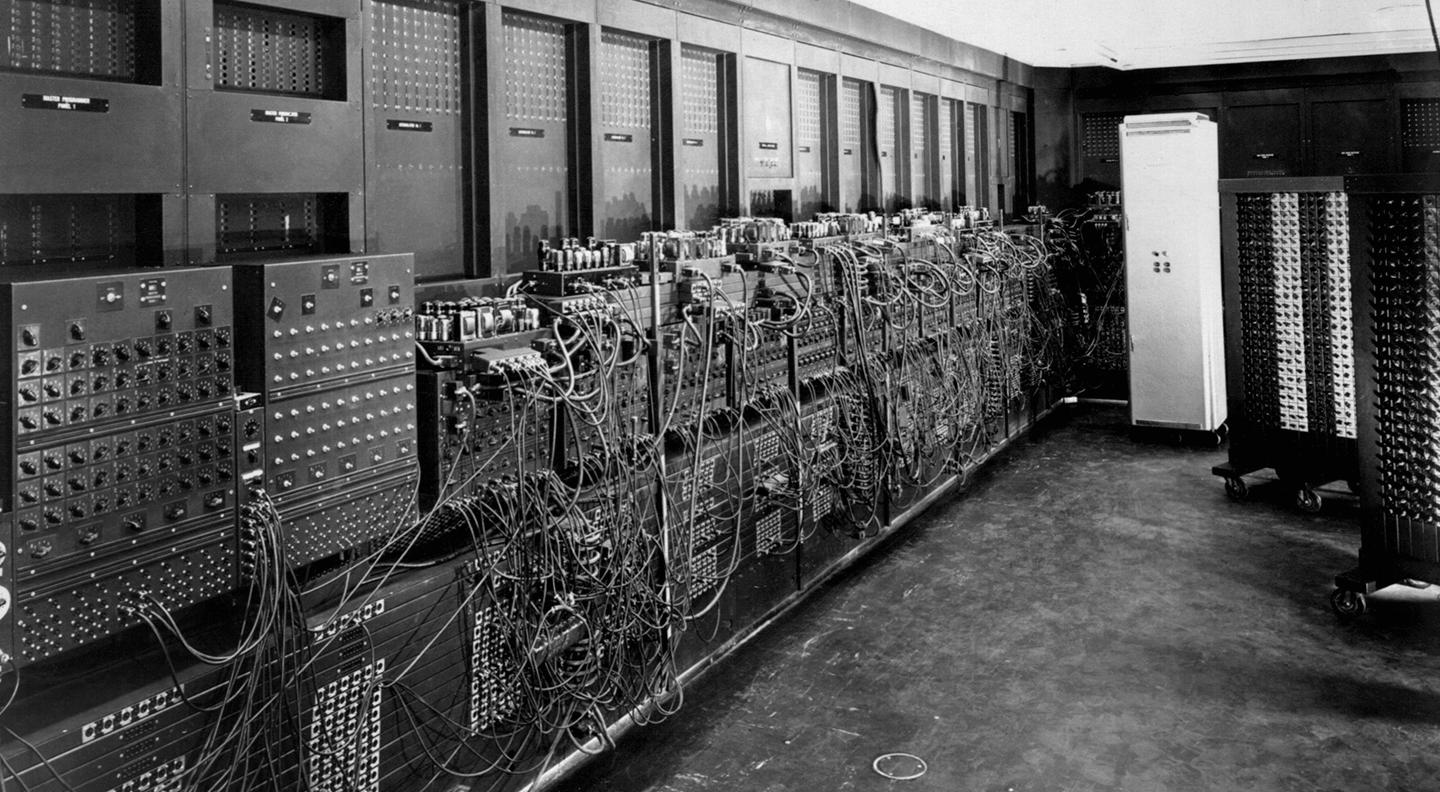
\includegraphics[
	width=0.75\textwidth,
	height=4cm,
	keepaspectratio
	]{images/5.jpg}
\end{block}

\begin{block}{但是}
	这时的电子计算机尚未拥有现代意义上的操作系统，程序的装载、准备和运行需要大量人工参与，十分复杂。
\end{block}

\end{frame}


\begin{frame}{操作系统发展史}
	
	\begin{block}{真的需要那么多人工参与吗？}
		\hspace*{2em}假设我们有100个计算任务，如果每完成一个任务，都需要工作人员手动准备下一个任务，不仅麻烦，还会让昂贵的计算机白白等待。
	\end{block}
	
	\vspace{0.3cm}
	
	\begin{block}{能不能让计算机自己工作呢？}
		\hspace*{2em}能不能提前把任务准备好，让计算机完成一个任务后，自动开始执行下一个任务呢？
		
		\centering
		任务一 $\longrightarrow$ 任务二
		$\longrightarrow$ 任务三
		$\longrightarrow$ $\cdots$
	\end{block}
	
	\begin{block}{单道批处理系统（Simple Batch System）}
		\hspace*{2em}20 世纪 50 年代，批处理系统逐渐出现。它能够自动组织并依次执行一批作业，减少人工干预，提高计算机的使用效率，但此时的批处理系统，还是一次只运行一个作业。
	\end{block}
	
\end{frame}

\begin{frame}{操作系统发展史}
	\begin{figure}
		\centering
		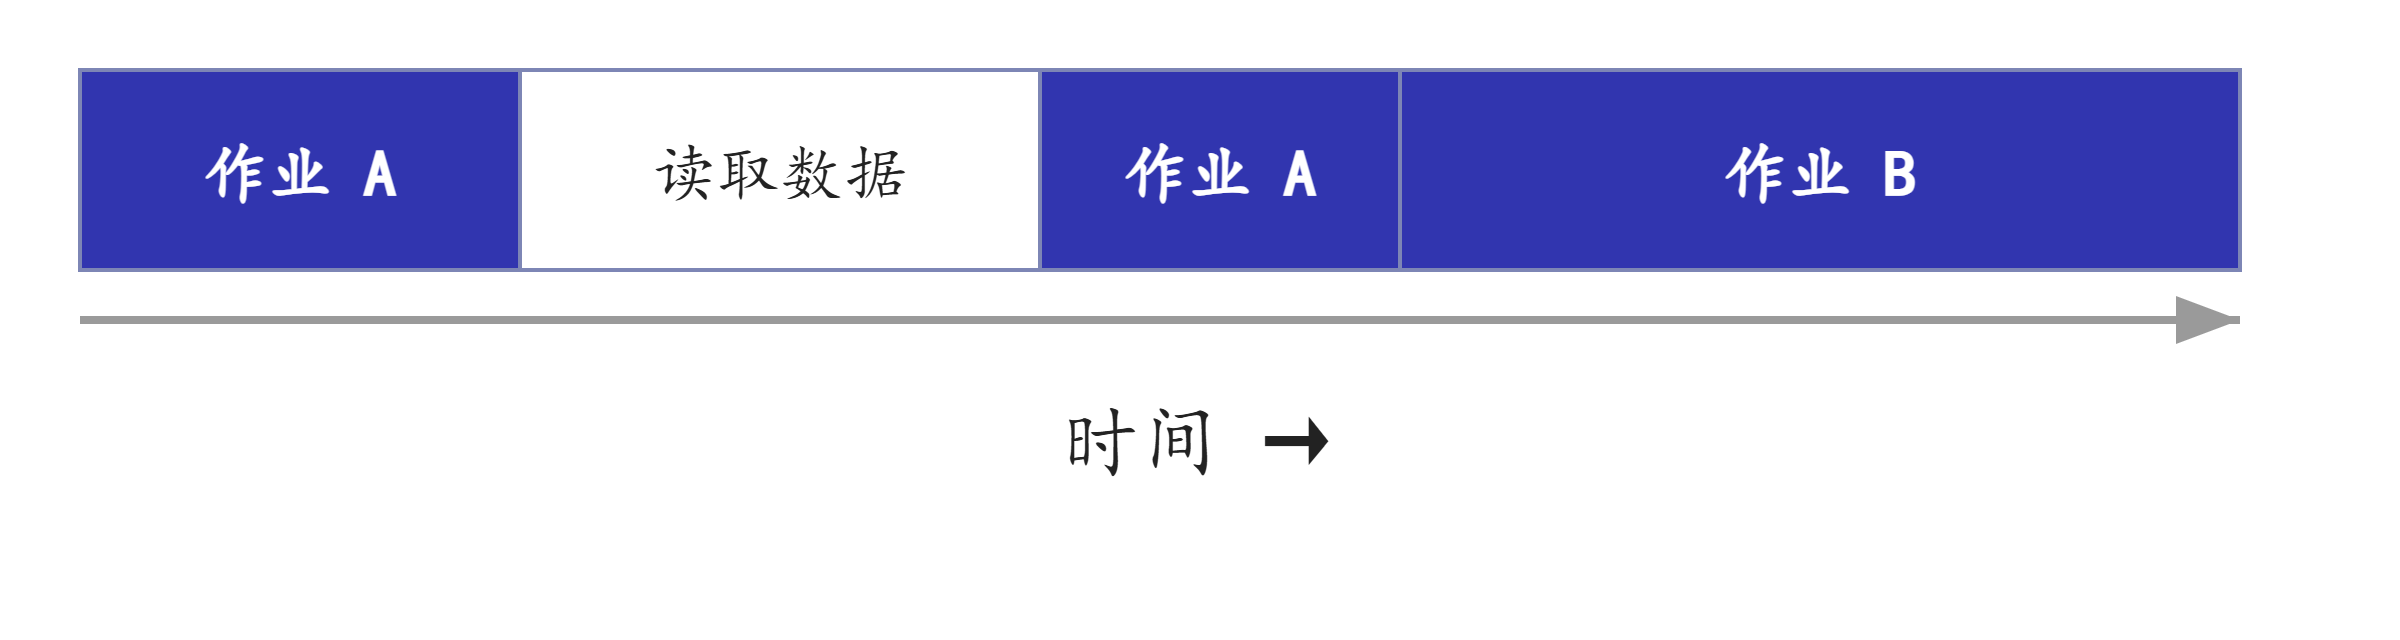
\includegraphics[width=0.7\textwidth]{images/6.png}
		\caption{单道批处理}
	\end{figure}
\begin{figure}
	\centering
	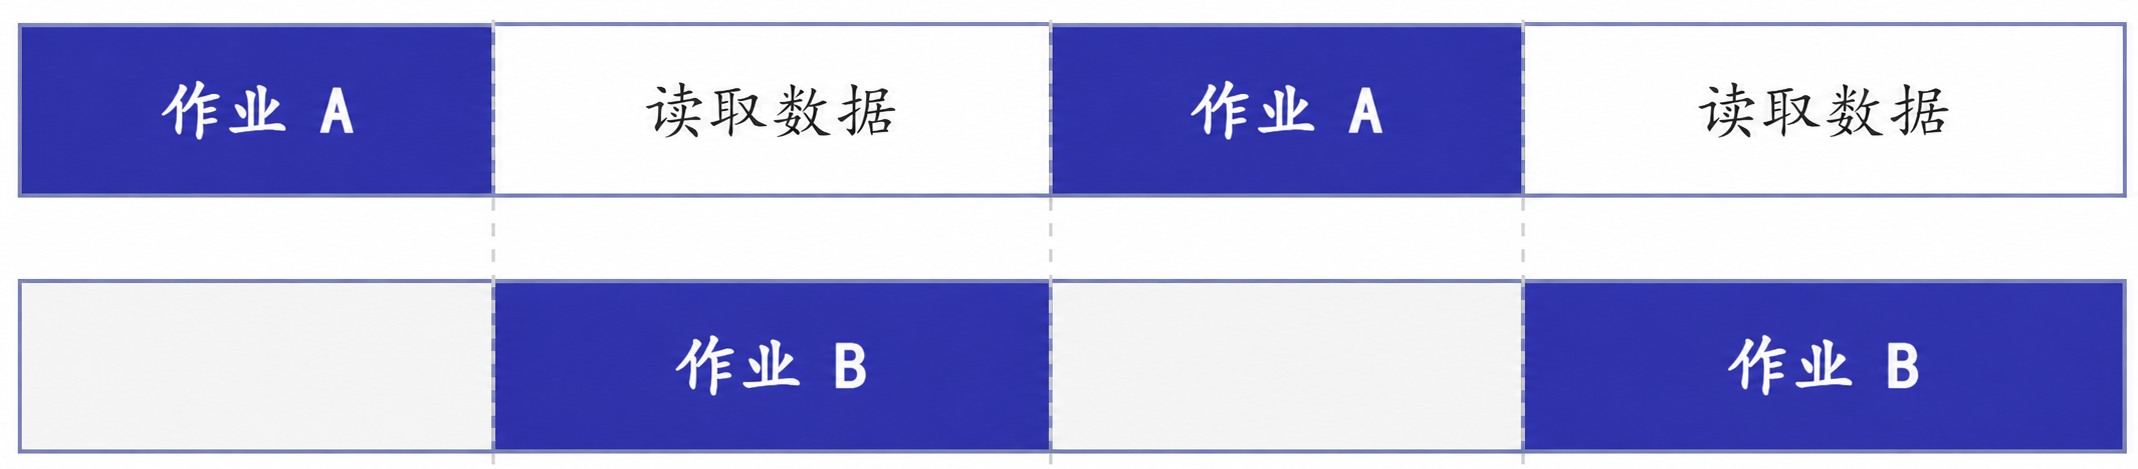
\includegraphics[width=0.7\textwidth]{images/7.png}
	\caption{多道批处理}
\end{figure}

\end{frame}

\begin{frame}{操作系统发展史}
\begin{block}{分时操作系统（Time-Sharing System）}
	\hspace*{2em}批处理系统虽然提高了计算机的使用效率，但用户提交作业后，往往需要等待才能得到结果，难以直接与计算机交互。
	\par\hspace*{2em}20 世纪 60 年代，分时操作系统逐渐发展起来。它通过时间片等调度机制，让多个用户的程序轮流使用处理器，使每个用户都能通过终端与计算机交互，并获得较为及时的响应。
\end{block}
\begin{figure}
	\centering
	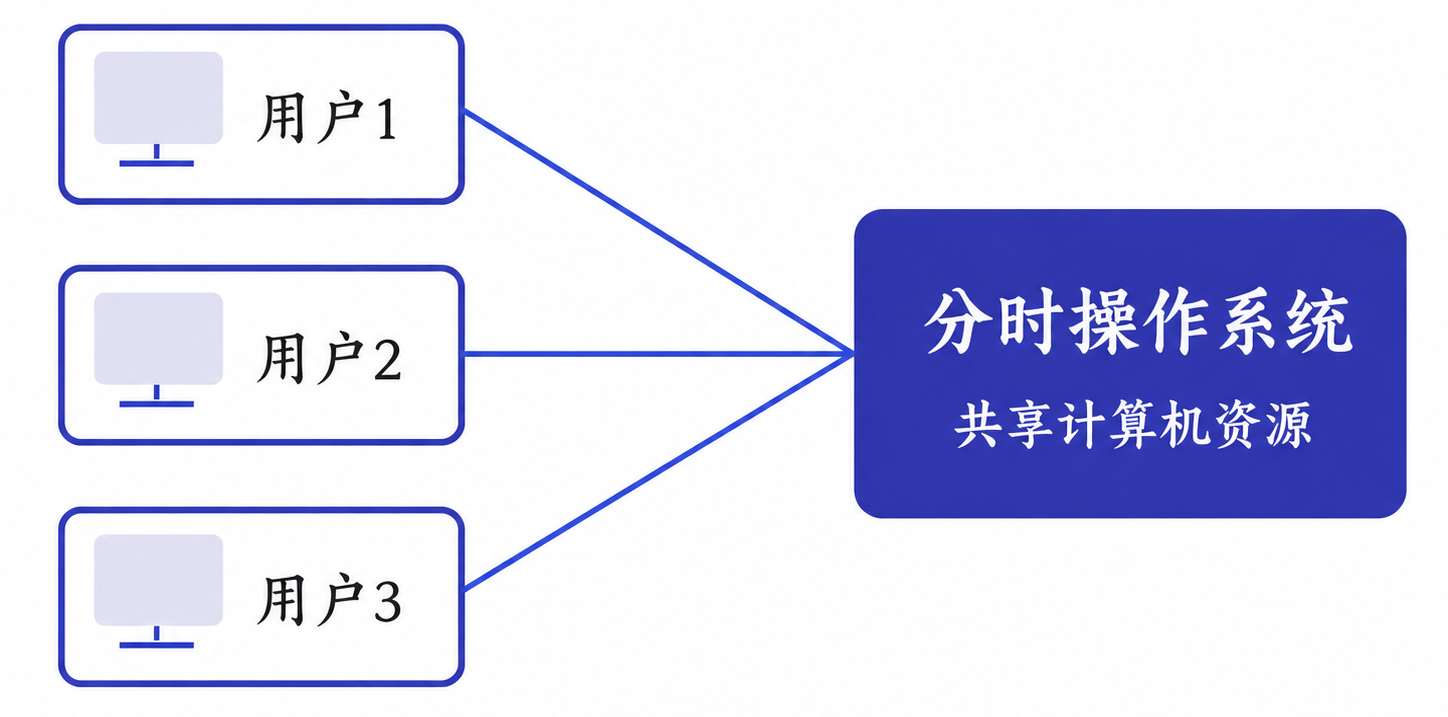
\includegraphics[width=0.45\textwidth]{images/8.png}
\end{figure}
\end{frame}

\begin{frame}{操作系统发展史}
\begin{block}{话说贝尔实验室}
\hspace*{2em}20 世纪 60 年代，MIT、贝尔实验室与通用电气公司合作开发了一套名为 Multics 的分时操作系统。但是，随着系统越来越复杂，开发难度和成本也越来越高，开发进度不及预期，最后贝尔实验室退出了该项目。
\end{block}
\begin{block}{能不能简单一些呢？UNIX！}
\hspace*{2em}贝尔实验室的研究人员充分吸取了经验教训，不追求一开始就实现大量复杂功能，而是先构建一套小巧、实用、可以不断扩展的系统，也就是后来的UNIX。
\begin{itemize}
	\item 多用户：允许多个用户通过终端共享计算机资源
	\item 简洁性：使用层次化文件系统，
	通过 Shell 和各种小工具完成复杂任务
	\item 可移植性：系统不必完全依赖某一种计算机硬件
\end{itemize}
\end{block}
\end{frame}


\begin{frame}{操作系统发展史}
	
	\begin{block}{UNIX 走出实验室}
		\hspace*{2em}凭借优秀的设计与良好的可移植性，UNIX 逐渐从研究机构走向大学与商业市场，吸引了越来越多的开发者和企业参与。
		
		\par\hspace*{2em}早期的一些大学和研究机构甚至能够获得 UNIX 的源代码，研究它的工作原理，并在许可范围内改进它。
	\end{block}
	
	\begin{block}{好景不长}
		\hspace*{2em}为了获得竞争优势，不同厂商纷纷为自己的UNIX系统增加独有的功能和接口。这些系统虽然都属于UNIX家族，却不一定能兼容彼此的软件。
		\begin{itemize}
			\item 对开发者：同一个程序可能需要针对不同的UNIX系统进行反复修改和适配
			\item 对用户：更换系统可能意味着高昂的迁移成本，以及对特定的厂商的依赖
		\end{itemize}
		\par\hspace*{2em}\alert{各大厂商围绕技术标准与商业利益陷入了纷争}
	\end{block}
\end{frame}




\begin{frame}{从 UNIX 到自由软件}
	
	\begin{block}{能不能换一种方式？}
		\hspace*{2em}既然 UNIX 的设计已经如此成熟，我们为什么不能从头开发一套类似的操作系统，不再依赖商业 UNIX 的专有源代码呢？	
	\end{block}
	
	\begin{block}{GNU 计划（GNU Project）}
		\hspace*{2em}20 世纪 80 年代，Richard Stallman 发起了 GNU 计划，希望开发一套与 UNIX 兼容，但允许用户自由使用、研究、修改和分享的操作系统。
		
		\par\hspace*{2em}GNU 是``GNU's Not Unix'' 的递归缩写，意为“GNU 不是 UNIX”。
	\end{block}
	
	\begin{block}{自由软件（Free Software）}
		\hspace*{2em}GNU 计划不仅希望开发新的操作系统，更希望建立一种允许用户自由使用软件、研究源代码、分享改进成果的协作方式。
		
		\par\hspace*{2em}\alert{这里的“自由”并不是软件必须免费，而是用户对自己使用的软件享有基本自由。}
	\end{block}
	
\end{frame}


\begin{frame}{自由软件}
	\begin{block}{自由软件（Free Software）}
		\hspace*{2em}自由软件并不是指不收费的软件，而是指能够保障用户使用、研究、修改和分享软件等基本自由的软件。
	\end{block}
	\begin{block}{自由软件的四项基本自由(具体自由由具体许可证来决定)}
		\begin{itemize}
			\item 自由 0：出于任何目的运行软件的自由
			\item 自由 1：研究软件如何工作，
			并根据自己的需要修改软件的自由
			\item 自由 2：复制和再分发软件的自由
			\item 自由 3：向他人分发修改后版本的自由
		\end{itemize}
	\end{block}
	\begin{block}{自由不等于免费！}
		\hspace*{2em}假设你开发了一款软件，并将它以 100 元的价格出售，但允许购买者自由使用、研究、修改和分享它。\alert{那么，它仍然可以是一款自由软件！}
	\end{block}
\end{frame}

\begin{frame}{自由软件}
	\begin{block}{自由如何得到保障？}
		\hspace*{2em}假设我们开发了一款自由软件，允许所有人使用、修改和分享。
		\par\hspace*{2em}但如果有人修改了我们的软件，却不再向后来的软件使用者提供源代码，那么这些用户不就失去了研究和修改它的自由吗？
	\end{block}
	\begin{block}{Copyleft（著佐权）}
		\hspace*{2em}Copyleft 利用著作权与软件许可证，使自由软件在被修改和再分发时，仍然能够保持自由。\alert{自由不仅属于最初的用户，也应该属于后续的用户。}
	\end{block}
	\begin{block}{GNU GPL（GNU General Public License）}
		\hspace*{2em}为了实现Copyleft，GNU 计划推出了 GNU GPL。
		\par\hspace*{2em}GPL 允许用户使用、修改和分享软件，但如果将修改后的 GPL 软件分发给他人，就必须遵守相应的许可条件，使接收者继续享有这些自由，并按规定提供对应的源代码。
	\end{block}	
\end{frame}
\begin{frame}{从GNU到Linux}
	\begin{block}{GNU 已经做了很多事情}
		\hspace*{2em}GNU 计划并不只是提出了自由软件的理念，它还开发了许多重要的软件工具。
		\par\hspace*{2em}例如，编译程序可以用到 GCC，命令行交互可以用到 Bash，日常文件操作也有许多 GNU 工具支持。
	\end{block}
	\begin{block}{但还缺少一个关键部分}
		\hspace*{2em}如果想真正构建一套完整的操作系统，仅有编译器、命令行工具和基础软件还不够。
		\par\hspace*{2em}我们前面说过，操作系统要负责管理处理器、内存和设备，完成这些底层工作的核心部分，就是\alert{内核（Kernel）}。而当时，GNU 还没有一个成熟可用的内核。
	\end{block}
\end{frame}

\begin{frame}{Linux 的诞生}
	\begin{block}{一个大学生的个人项目}
		\hspace*{2em}20 世纪 90 年代初，芬兰赫尔辛基大学的学生 Linus Torvalds在学习和使用类 UNIX 系统的过程中，对操作系统的工作原理产生了浓厚的兴趣。
		\par\hspace*{2em}于是，他决定动手为自己的计算机开发一个操作系统内核，这就是后来 Linux 的起点。
	\end{block}
	\begin{block}{一条改变历史的网络留言}
		\hspace*{2em}1991 年，Linus 在互联网上介绍了自己的项目，并向其他开发者征求意见。
		\par\hspace*{2em}他甚至在留言中表示，这只是一个业余项目，不会像 GNU 那样庞大和专业。
	\end{block}
\end{frame}

\begin{frame}{GNU 与 Linux 的相遇}
	\begin{block}{两个项目，各有所长}
		\hspace*{2em}GNU 计划已经开发出了编译器、Bash、基础命令等大量系统工具，但自己的操作系统内核尚未成熟。
		\par\hspace*{2em}而 Linux 已经拥有了能够管理计算机硬件资源的内核，却还需要其他系统工具，才能构建一套方便用户使用的操作系统。
	\end{block}
	
	\begin{block}{GNU/Linux 的诞生}
		\hspace*{2em}开发者逐渐将 Linux 内核与 GNU 工具及其他系统组件结合起来，形成了一套实用的类 UNIX 操作系统。	
		\begin{center}
			GNU 系统工具
			$+$
			Linux 内核
			$+$
			其他组件
			
			$\Downarrow$
			
			\alert{GNU/Linux 操作系统}
		\end{center}
	\end{block}

\end{frame}

\begin{frame}{Linux 成为自由软件}
	\begin{block}{Linux 最初就是自由软件吗？}
		\hspace*{2em}Linux 最初就公开了源代码，允许其他开发者阅读和分享。但它最初的许可证明确禁止收费分发，即使仅仅收取手续费也不可以。
		\par\hspace*{2em}因此，早期 Linux 并不完全符合我们前面介绍的自由软件标准。
	\end{block}	
	\begin{block}{一项重要的决定：GNU GPL}
		\hspace*{2em}1992 年，Linus Torvalds 决定将 Linux 内核改为使用 GNU GPL 许可证。
		\par\hspace*{2em}从此，用户不仅能够研究、修改和分享 Linux，还可以在遵守许可证的前提下进行商业分发。
	\end{block}
\end{frame}


\begin{frame}{从个人项目到全球协作}
	
	\begin{block}{互联网让协作成为可能}
		\hspace*{2em}借助互联网，开发者可以通过讨论组、电子邮件等方式交流想法，并将代码修改整理成补丁（Patch），提交给项目的维护者。
		
		\par\hspace*{2em}经过讨论、审查和测试，合适的修改就有机会被合并到 Linux 中，让更多用户受益。
	\end{block}

	\begin{block}{开源不只是公开代码}
		\hspace*{2em}Linux的发展逐渐证明，一个大型软件项目不一定只能依靠某一家企业内部的开发团队。通过开放的许可、互联网以及有效的社区协作，来自不同地区的开发者也能够共同改进软件。\alert{一个人的项目，可以逐渐成为世界各地开发者共同参与的事业。}
	\end{block}
\end{frame}


\begin{frame}[t]{Linux 逐渐形成自己的生态}
	
	\begin{block}{如何让更多人使用 Linux？}
		\hspace*{2em}Linux 内核虽然已经能够管理计算机硬件，
		但普通用户还需要各种系统工具、程序库和应用软件。
		
		\par\hspace*{2em}如果每个人都要自己寻找这些软件，
		再逐个安装、配置，
		使用 Linux 的门槛仍然很高。
	\end{block}
	
	\vspace{0.3cm}
	
	\begin{block}{Linux 发行版（Linux Distribution）}
		\hspace*{2em}于是，开发者开始将 Linux 内核、
		GNU 工具以及其他必要的软件组织在一起，
		提供更加完整、方便安装和使用的操作系统。
		
		\par\hspace*{2em}20 世纪 90 年代，
		一批具有代表性的 Linux 发行版相继出现：
		
		\begin{itemize}
			\item Slackware：1993 年发布，注重简洁与稳定
			\item Debian：1993 年创立，强调自由软件与社区协作
			\item Red Hat Linux：1994 年推出早期测试版本，
			逐渐探索商业化应用
		\end{itemize}
	\end{block}
	
	\vspace{0.3cm}
	
	\begin{block}{从一个内核，到一个庞大的生态}
		\hspace*{2em}不同开发者可以围绕同一个 Linux 内核，
		根据各自的需求选择、整合和维护不同的软件，
		构建出面向不同用户的操作系统。
		
		\par\hspace*{2em}\alert{Linux 的发展逐渐证明：
			开放的软件不仅能够被共同改进，
			还能够成为更多创新的基础。}
	\end{block}
	
\end{frame}

\begin{frame}[t]{丰富多样的 Linux 发行版}
	
	\begin{block}{为什么会有这么多发行版？}
		\hspace*{2em}虽然不同的 Linux 发行版
		都以 Linux 内核为基础，
		但它们可以采用不同的系统工具、
		软件管理方式和更新策略，
		满足不同用户的需求。
	\end{block}
	\begin{columns}[T,onlytextwidth]
		
		\begin{column}{0.48\textwidth}
			
			\begin{block}{Ubuntu}
				基于 Debian，
				注重易用性，
				广泛应用于个人电脑、
				软件开发与服务器。
			\end{block}
			
			\begin{block}{Debian}
				由社区共同维护，
				重视软件自由与系统稳定性，
				也是许多其他发行版的基础。
			\end{block}
			
		\end{column}
		
		\begin{column}{0.48\textwidth}
			
			\begin{block}{Fedora}
				由开源社区推动，
				积极采用新的软件技术，
				提供桌面与服务器等版本。
			\end{block}
			\begin{block}{Arch Linux}
				强调简洁与高度可定制，
				采用滚动更新，
				适合喜欢自主配置系统的用户。
			\end{block}
			
		\end{column}
		
	\end{columns}
	\begin{center}
		\alert{同一个 Linux 内核生态，
			可以发展出满足不同需求的操作系统。}
	\end{center}
	
\end{frame}


\begin{frame}{从自由软件到开源软件}
	\begin{block}{时代正在发生变化}
		\hspace*{2em}随着计算机技术的发展，个人计算机逐渐普及，越来越多的普通人拥有了编写软件的条件。与此同时，互联网的发展让世界各地的开发者能够方便地交流代码、分享成果，甚至共同开发同一个软件项目。
	\end{block}
	\begin{block}{开放协作的价值逐渐显现}
		\hspace*{2em}自由软件的发展让人们逐渐认识到，开放源代码不仅能够保障用户的自由，还能汇聚不同开发者的力量，共同改进软件。1998 年，一部分软件界人士开始推广“开源软件”这一名称，希望强调开放协作的实际价值，吸引更多开发者和企业参与。
	\end{block}
	\begin{block}{两种理念，共同推动软件发展}
		\begin{itemize}
			\item 自由软件：更强调用户应当拥有的基本权利
			\item 开源软件：更强调开放协作带来的实际价值
		\end{itemize}
	\end{block}
\end{frame}

\begin{frame}{开源的意义}
	\begin{block}{假如一位学长开发了一款校园软件……}
		\hspace*{2em}一位学长开发了一款非常实用的课表管理软件，但毕业后没有时间继续维护。后来的同学发现了问题，还希望增加新的功能。难道这个软件就只能停止更新了吗？
	\end{block}
	\begin{block}{如果这是一款开源软件呢？}
		\begin{itemize}
			\item 知识共享：其他人可以阅读源代码，学习软件的实现原理
			\item 协作创新：不同开发者可以共同修复问题、增加功能，并分享改进成果
			\item 自主维护：即使原作者不再维护，其他人仍有权继续开发这个项目
		\end{itemize}
	\end{block}
	\begin{block}{开源的价值}
		\hspace*{2em}开源不仅是公开代码，更是通过开放的许可与协作，让更多人有机会参与软件的学习、改进与长期发展。
		\par\hspace*{2em}\alert{让创新不止于一个人，让技术能够被更多人共同推动。}
	\end{block}
\end{frame}

\begin{frame}{开源的意义}
	\begin{block}{开源的意义}
		\hspace*{2em}开源无法消除所有的不平等，但它能够降低技术的获取门槛，打破部分知识壁垒，让更多人有机会参与技术的发展。
		\par\hspace*{2em}\alert{技术进步不应只是少数人的事业，更多人也应该有机会成为创造者。}
	\end{block}
\end{frame}



\begin{frame}
	\title{谢谢大家}
	\subtitle{第一讲：从操作系统到开源}
	\author{潘宇琦\hspace*{1em}申鹏威}
	\date{2026年10月}
	\titlepage
\end{frame}

	
\end{document}